\section{Related Work}
\label{sec:related}
\subsection{Artificial Intelligence Techniques - Neural Networks}
\label{sub:aiml}
In this section we will describe common Artificial Intelligence (AI) techniques used in models for  facial expression recognition (Section \ref{sub:rw_fer}).
\subsubsection{Neural Networks}
A \emph{Neural Network NN} is built with many \emph{neurons}, which are connected by \emph{activators} that have a \emph{weight}. These neurons are located in many layers which give structure to the NN \cite{schmidhuber2015deep}. The first layer of the NN is the so-called \emph{input layer}, which acts as the entry point for the data that is to be analysed. The last layer is defined as the \emph{output layer}. It contains the information about the estimation that the NN has made. The in-between layers are called \emph{hidden layers}.

A NN can also be represented as a very complex function $f(x) = y$, where $x$ represents the input, and $y$ the computed output (the prediction).

Shallow NN consist of few hidden layers, and have been a topic for a long time. The discovery of \emph{backpropagation} allowed the development of NNs with many hidden layers, called \emph{Deep Neural Networks DNN} \cite{schmidhuber2015deep}.

\subsubsection{Convolutional Neural Networks CNN}
CNNs lend themselves well to tasks in \emph{Computer Vision CV} \cite{albawi2017understanding}. Most importantly, they reduce the amount of parameters, while also emphasizing locality and context of the input information. This enables edge detection, shape detection, and object detection in successive layers of a deep CNN, which will be especially helpful in models (Section \ref{sec:models}) that analyse faces and their active Action Units (Section \ref{subsub:au}).

Subsequent convolutional layers, coupled with pooling layers, enable the detection of more and more complex structures. While the initial layers might detect straight edges, the following layers will recognize compound structures, and ultimately features like raised eyebrows (AU 1 and/or AU 2).

\subsubsection{Temporal Neural Networks with Gated Recurrent Units GRU}
The previously described NNs can be described as \emph{feedforward} NNs. The direction of information flow is linearly through input, hidden and to the output layer. This can be contrasted with \emph{feedback} NNs, that have mechanisms that allow for 'memory' in a NN \cite{wang2003artificial}. These \emph{Recurrent Neural Networks RNN} enable the analysis of temporal data.

A concrete implementation for a temporal recurrent layer are \emph{Gated Recurrent Units GRU} proposed by Cho et al. \cite{cho2014properties} \cite{chung2014empirical}. GRUs act similarly to \emph{Long Short Term Memory LSTM} \cite{hochreiter1997lstm} layers, while removing memory gates \cite{chung2014empirical}. Empirical research has shown that GRUs can be more performant than LSTMs in less frequent datasets \cite{gruber2020gru}.

\subsection{Emotional Models from Facial Expression}
\label{sub:rw_fer}
\subsubsection{Categorical Model}
One of the most recognized ways to separate emotional states in non-verbal communication is presented by Paul Ekman \cite{ekman1987universals} \cite{ekman2013emotion}. His research postulates a cross-cultural agreement in judging facial expressions \cite{ekman1987universals}. Basic emotion theory assumes a fixed amount of human emotions, which is also believed and postulated by Ekman and Russell \cite{ekman1992basic} \cite{russell2006}. Ekman proposes a split into seven categories: anger, happiness, surprise, sadness, fear, disgust and contempt. He later consolidated them down to six, removing contempt. 

\subsubsection{Dimensional Model}

Dimensional systems use a set of dimensions, \emph{valence}, \emph{arousal} and in some cases \emph{dominance} to estimate the affective state of a person. James A. Russell introduced the two dimensional circumplex model of affect \cite{russell1980circumplex}, where he mapped emotions in the valence-arousal space. Valence represents the (un-)pleasantness of an affective state, and arousal represents the activation. \cite{posner2005circumplex}. The emotions from the categorical have their place in this dimensional field, e.g. happy having a high score for valence and arousal.

\begin{figure}
    \centering
    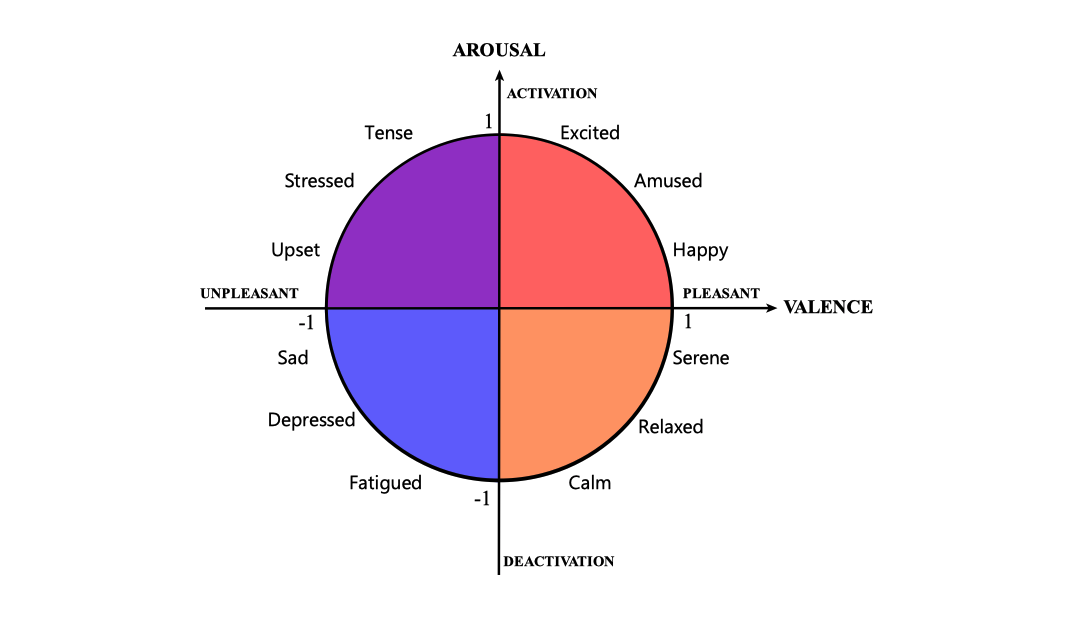
\includegraphics[width=0.8\textwidth]{res/circumplex.png}
    \caption{The circumplex model of affect with the valence and arousal axis with selected emotions. \cite{russell1980circumplex} \cite{pourmirzaei2021an}}
    \label{fig:circumplexImg}
\end{figure}

\subsubsection{Action Units}
\label{subsub:au}

Introduced by Hjortsjö \cite{hjortsjo1969man} and further refined by Ekman \cite{friesen1978facial}, the \emph{Facial Action Coding System FACS} tries to separate and classify facial movements that lead to distinct facial expressions. Combinations of the 28 \emph{Action Units AUs} can then be used to describe an affective expression.

\begin{table}[]
    \centering
    \begin{tabular}{c|c}
       \textbf{Emotion}  & \textbf{Action Units} \\ \hline
        Happy & 12, 25 \\
        Sad & 4, 15 \\
        Fearful & 1, 4, 20, 25 \\
        Angry & 4, 7, 24 \\
        Surprised & 1, 2, 25, 26 \\
        Disgusted & 9, 10, 17
    \end{tabular}
    \caption{The basic emotions with their corresponding prototypical AUs \cite{fabian2016emotionet}}
    \label{tab:emotionAUs}
\end{table}

\subsection{Automatic Facial Emotion Recognition}
Facial Emotion Recognition FER can be divided into two different groups: conventional and Deep-Learning-based. \cite{ko2018brief}

Conventional FER systems work in a pipeline that consists of three steps: face detection, feature extraction and expression classification \cite{ko2018brief}.

The deep learning approach has established itself as the state-of-the-art method for FER models. In contrast to the handcrafted conventional pipeline, the more modern approach enables an end-to-end learning method \cite{ko2018brief}. The most prominent model-type in FER is the convolutional neural network CNN. CNN-based networks offer themselves very well to image processing, which make them a great candidate for FER systems. 

Deep learning models can further be divided into two categories. The first one outputs emotions directly from the model \cite{ebrahimi2015recurrent} \cite{kim2017multi} \cite{jung2015joint}, where the second one classifies AU activations, from which emotions can be deduced \cite{breuer2017deep} \cite{zhao2016deep} \cite{chu2017learning}. 

\subsection{Phonemes and Visemes}
The content of an act of speech can be segmented into words, syllables, and \emph{phonemes} \cite{savin1970nonperceptual}. Languages differ in their amount of phonemes, with the New Guinean language Rotokas having 11, whereas the Namibias !Xóõ is using 160. English, the primary language we're be looking at in this thesis, has 37-41 phonemes, differing by dialect \cite{Hayes2009}. Phonemes are very important in FER. A speaking subjects face, and activated AUs, will be influenced by the lexical content of their speech, which is defined by the current phoneme. The face of a person in the act of pronouncing a phoneme will have a certain look to it. Several phonemes can be grouped together based on the distinct look they produce. These groups are called \emph{visemes}. There are several different phoneme-to-viseme mappings in research, with no concrete agreement on a 'best mapping' \cite{cappelletta2012viseme}.

Visemes are particularly interesting for us, since our research is purely based in the visual domain. Differences between phonemes that are purely audiocentric are of no relevance for us. A viseme mapping reduces the categories for visually based lexical content, which makes building and training models easier.